\section{Generic \sysname{} design}
\label{sec:generic}

In addition to Clos networks, prior literatures have proposed different data center
network topology. In this section, we show that \sysname{} can be extended to
support generic topology and routing. In addition, unlike the prior section focusing 
on high-level ideas, we will formalize the expression of \sysname{}. This is necessary
for explaining the algorithm without specific topology properties.

After removing the Clos-specific mechanisms, here is a brief description of 
generic \sysname{}.

%We briefly describe the generic implementation of \sysname{}. The implementation 
%is described in detail in \S\ref{sec:implementation}.

\sysname{} works by tagging packets.  A packet arrives at the ingress port $i$
of a switch $S$ with a tag $j$. The arriving packet packet is enqueued in ingress 
queue $j$.  At departure, based on the values of $i$, $j$ and egress port, 
the packet is possibly given a new tag, say $k$. In this case, the packet is put 
into egress queue $k$. The rest of the forwarding pipeline, as well as PFC 
PAUSE/Resume behavior (\S\ref{sec:background}) operates without change. 

The smartness of the system lies in generating the tag changing rules: based on 
ingress port, incoming tag and egress port, the switch must decide whether to change
the tag, and what the new tag value is. In Clos version \sysname{}, we leverage
our knowledge of Clos and find that tagging on bounce is a good solution. 
Similar to the Clos version \sysname{}, we use the topology and {\em lossless routes} 
as input to generate these rules for generic topology.
The rules generation is based on similar ideas as for Clos network.  

%\sysname{} does not require any changes to the topology of the network or the
%routing. However, our  key insight is that we can take the topology and the
%routes that must be lossless (we call them {\em lossless routes}) as input, and
%use them to generate the mappings described earlier. 


%First, the switch configurations eliminate deadlock by reacting to the past path of each packet
%and move the packet into a safe priority just before CBD may appear.  Second,
%the transition of priority is designed carefully so that  a single tag in the
%packet header is sufficient for each switch to make such decisions. Finally, we
%make sure that \sysname{} requires only a small number of lossless queues. We
%now describe these ideas in detail.

\subsection{Definition of A Tagging Scheme}

Before we get to the detailed designs, we first formalize the tagging scheme.
Let $A_i$ represent a unique ingress port in the network, {\em i.e.,} switch $A$'s $i^{th}$ ingress port.
We use a {\em tagged graph} $G(V,E)$ to uniquely represent a tagging scheme.
Given a tagging scheme, the {\em tagged graph} $G(V,E)$ is generated following below rules.

\begin{enumerate}
\item $G$ contains a node, $(A_i, x)$, {\em iff.} a port $A_i$ may receive packets with tag $x$, and these packets must 
be lossless. $V$ is the set of all such nodes.
\item In $G$, there exists an edge $(A_i, x)\rightarrow(B_j, y)$ {\em iff.} switch $A$ and $B$ are 
connected, {\em and} switch $A$ may change a packet's tag from $x$ to $y$ before sending to $B$ (the case $x=y$ also counts).
$E$ is the set of all such edges.
\end{enumerate}

The tags define a partition of the tagged graph, $\{G_k\}$, whose nodes are $V(G_k) = \{(A_i,
k) | \forall A, i\}$ and edges are $E(G_k) = \{v_0 \rightarrow v_1 | \forall v_0, v_1 \in V(G_k) and v_0 \rightarrow v_1 \in E(G)\}$
Each $G_k$ is mapped to a unique
lossless priority.  Each node is an ACL rule to match on a tag on an ingress port, and
assign corresponding lossless queue.  In addition, each edge corresponds 
to a switch action of setting the tag for the next hop at the egress.

\begin{table}
\small
\centering
\begin{tabular}{|c|c|}
\hline
Symbol & Description \\ \hline
$A_i$ & Switch $A$'s $i^{th}$ ingress port  \\ \hline
$(A_i, x)$ & A node in tagged graph \\ \hline
$(A_i, x)\rightarrow(B_j, y)$ & A tagged edge \\ \hline
$V$ & All tagged nodes  \\ \hline
$E$ & All tagged edges \\ \hline
$G(V, E)$ & Tagged graph \\ \hline
\end{tabular}
\caption{Notations in the formalized description.}
\label{tab:symbols}
\end{table}

\para{Handling packets that do not follow the lossless routes.}
If a packet does not match any edges in $G(V,E)$, it means the packet is not 
expected in the lossless routing.
Such packets are assigned a special tag, and all switches match on this tag and 
assign lossy priority. This rule sits at the bottom of switch egress ACL, acting 
as a default safeguard that avoids unexpected buffer dependency.

To guarantee deadlock-free, we directly extend the properties described 
in \S~\ref{subsec:combine} to two requirements of $G(V,E)$. First, any 
$G_i$ does {\em not} have a cycle. This is because each edge in $G_i$ is 
essentially a buffer dependency -- whether $A_i$ can dequeue packets depending on whether
$B_j$ has paused upstream. A cycle in $G_i$ means cyclic buffer dependency.
Second, there is no link going from $G_i$ to $G_j$ if $i>j$. 
This means we enforce the order of $G_i$.

\subsubsection{Proof of deadlock freedom}

\begin{theorem}
Any tag system, defined by $G(V,E)$, that satisfies the above two requirements is deadlock-free.
\end{theorem}

\begin{proof}
We prove by contradiction. Suppose there exists a tag system,
whose $G(V,E)$ satisfies the above two requirements, but is not deadlock-free. This means
$G(V,E)$ has a cycle $v_0 \rightarrow v_1 \rightarrow ... \rightarrow v_0$. With certain 
traffic that covers all hops in the circle, the cycle turns into a CBD and can form deadlock.

\textbf{Case 1:} All the nodes in the cycle has the same tag $t$. According to
the first requirement, $G_t$ does {\em not} have a cycle. Contradicted.

\textbf{Case 2:} The nodes in the cycle have at least two different tags, $t_0$ and $t_1$.
Without loss of generality, we assume $t_0 < t_1$, and $v_i$ has tag $t_0$, $v_j$
has tag $t_1$. Because $v_i$ and $v_j$ belongs to a circle, there must exists 
a path going from $v_j$ to $v_i$. Since $t_0 < t_1$, there must exist a hop where
the tag decreases. However, according to the second requirement, such hop cannot
exist. Contradicted.

Case 1 and Case 2 cover all possible scenarios. Thus, we conclude that there does not 
exist a $G(V,E)$ that satisfies the two requirements but is not deadlock-free.
\end{proof}

%\textbf{Proof sketch:} We prove by contradiction. Suppose we can find a topology and a
%set of lossless routes, for which there exists a subspace partition and priority
%transition that satisfies the above two requirements, but is not deadlock-free.
%Then, as the tag system is not deadlock-free, we can find a set of micropaths
%that form a CBD. 



%\textbf{Case 2:} These micropaths are in different subspaces. We sort these
%micropaths according to the subspaces they belong to, and choose a micropath in
%the smallest subspace. Since these micropaths can form a CBD,  starting from the
%source end of the chosen micropath, we can always find a circular path back to
%the chosen micropath when traversing along these micropaths. 
 
%According to requirement 1, once we enter a larger subspace, we can never go
%back. So this circular path should only include micropaths in the smallest
%subspace. But according to requirement 2, micropaths within the same subspace do
%not form a CBD. Hence no circular path can be found within the smallest
%subspace. So this circular path does not exist. Contradicted.
 
%Thus, we conclude that there do not exist a set of micropaths that form a CBD.
%This contradicts the supposition that the tag system is not deadlock-free.
%Hence, any tag system that satisfies the above two requirements is
%deadlock-free.


\subsection{Step 1: Deadlock-free Tags} 

\begin{figure*}[t]
	\centering
	\subfloat[short for lof][Input topology and lossless routes.] {
		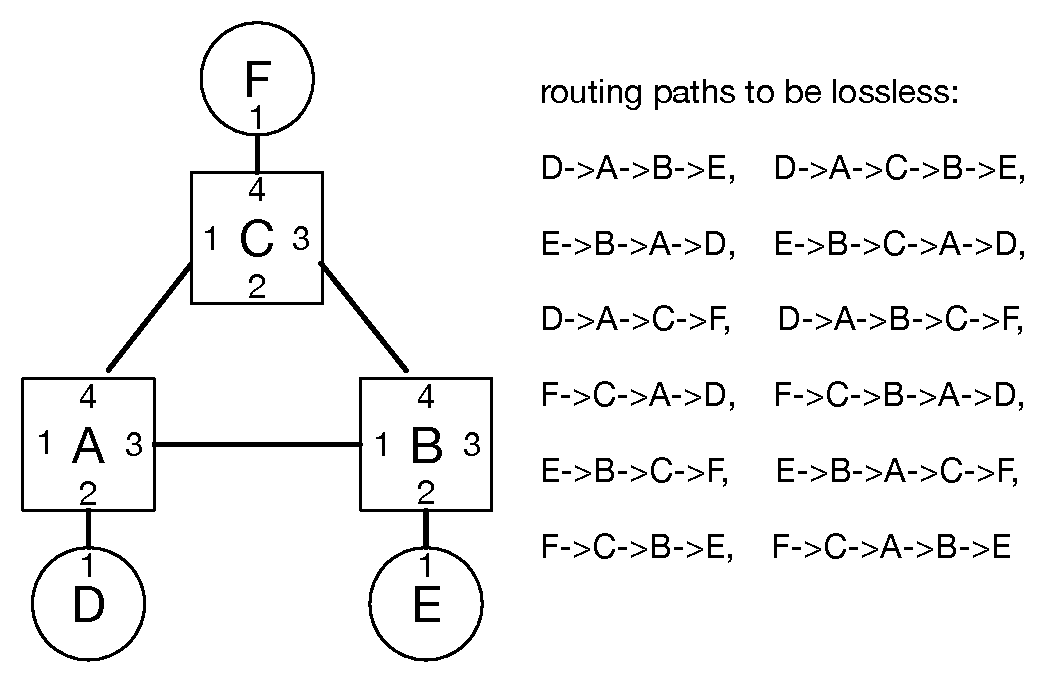
\includegraphics[width=0.6\textwidth] {figs/alo_walkthrough_a}
	}
	\subfloat[short for lof][Output tagged graph.]{
		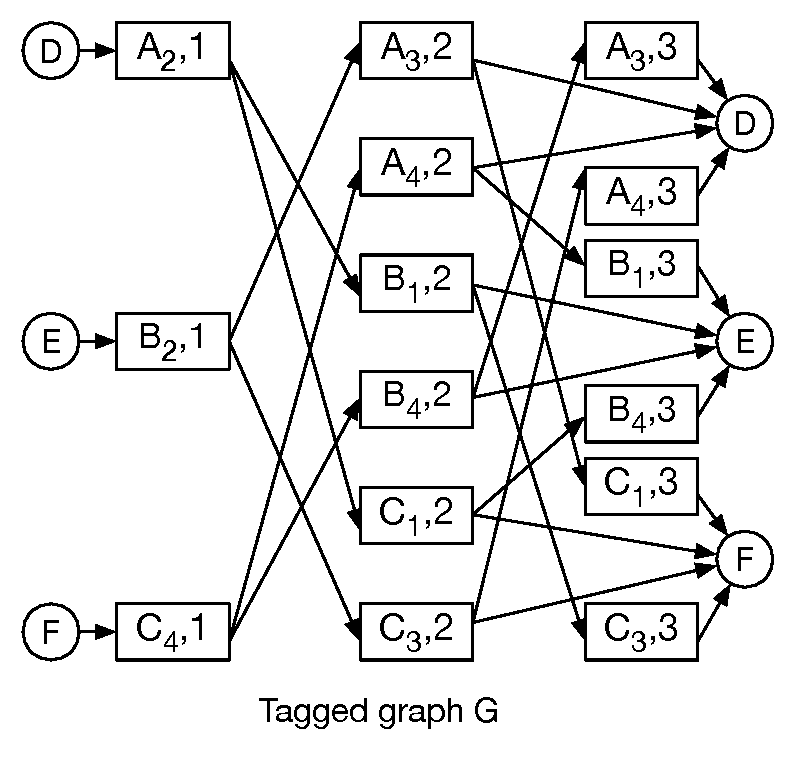
\includegraphics[width=0.4\textwidth] {figs/alo_walkthrough_b}
	}
	\caption{The input and output of Algorithm~\ref{alg:ttl}.}\label{fig:three_node}
\end{figure*}

Like the Clos version \sysname{}, we will first design a tagging scheme that avoids
deadlock, then combine tags to reduce the required lossless queues. 
For general graph without structure information, a straight forward tagging 
system is to monotonically decrease the tag (thus, the priority) every hop, as described in 
Algorithm~\ref{alg:ttl}. 

\begin{algorithm}
	\small
    \KwIn{Topology and lossless routes $R$}
	\KwOut{A tagged graph $G(V, E)$}
	$V \gets Set()$\;
	$E \gets Set()$\; 
	\For{each path $r$ in $R$} {
		$tag \gets 0$\;
		\For{each hop $h$ in $r$} {
			$V \gets V \cup \{(h, tag)\}$\;
			$E \gets E \cup \{lastHop\rightarrow(h, tag)\}$\;
			$tag \gets tag+1$\;
		}
	}
	\Return{$G(V, E)$}\;
    \caption{A brute-force tagging system that decreases the tag by one every hop.}
	\label{alg:ttl}
\end{algorithm}

It is easy to verify that the above requirements are met\fixme{may need to elaborate}, so 
deadlock is eliminated with this tagging system. However, it requires 
too many tags (lossless queues) in a large network since it depends on the diameter of the topology.

We use a three node topology as an example to demonstrate the input and output of the 
algorithm, as shown in Figure~\ref{fig:three_node}. It will require {\em four} 
tags, since the longest path length is four.

\fixme{This idea appeared in prior work. However, it is a special case in our tagging system,
and has the drawback that it requires too many lossless queues. Here we give it a formal 
expression in our framwork, and will further optimize it in the next section.}


%% Section~\ref{sec:greedy} shows a way to achieve this.  Inevitably, we will need
%% {\em multiple} switch lossless queues to support one lossless application class.
%% Specifically, we divide the buffer of network nodes into $k$ partitions, and let
%% the $j$-$th$ partition associated with priority queue $j$. If a packet is
%% classified into priority queue $j$, it will be buffered in the $j$-$th$ buffer
%% partition and can generate PFC of priority $j$.  In this section, we focus on
%% supporting {\em just one} lossless application class. In
%% Section~\ref{sec:specific}, we will revisit this issue and show how we may
%% support multiple application classes more efficiently.

\para{The counter-part in the Clos version.} To ease the comparison, we show the tagging
scheme of Clos in Algorithm~\ref{alg:clos}. The only difference is where the tag
is updated. It is due to the fact that we have more knowledge of Clos, a structured topology.
Algorithm~\ref{alg:clos} already includes the idea of combining tags (\S\ref{subsec:combine}),
so the algorithm in the next section will not further optimize the output.

\begin{algorithm}
	\small
    \KwIn{Clos topology and lossless routes $R$}
	\KwOut{A tagged graph $G(V, E)$}
	$V \gets Set()$\;
	$E \gets Set()$\; 
	\For{each path $r$ in $R$} {
		$tag \gets 0$\;
		\For{each hop $h$ in $r$} {
			$V \gets V \cup \{(h, tag)\}$\;
			$E \gets E \cup \{lastHop\rightarrow(h, tag)\}$\;
			\If{$h$ is up-facing \&\& nextHop is down-facing} {
				$tag \gets tag+1$\;
			}
		}
	}
	\Return{$G(V, E)$}\;
    \caption{The optimal tagging system for Clos topology.}
	\label{alg:clos}
\end{algorithm}



%\subsection{Idea 2: Tag for Ordered Micropath Subspaces}\label{sec:tag_order}

%By properly dividing lossless routes into multiple subspaces of micropaths, we
%can ensure that CBD is eliminated {\em within} each subspace. We will discuss
%the details of the algorithm are described later in this section. But first, we
%must consider another issue: Even though proper micropath partition ensures no
%CBD {\em within} each priority, packets can still cause CBD {\em across}
%priorities, as shown in Figure~\ref{fig:subspace}(a). Switch must know the past
%path of each packet in order to decide the priority that avoids CBD. Obviously,
%the tag size is limited, so we can't carry the entire history of the packet in
%the tag. Thus, we need the next idea.

%As shown in Figure~\ref{fig:subspace}(b), we enforce the order of transitioning
%among micropath subspaces and tag only based on current subspace.  With this,
%the packets do not need to record the whole history of past micropaths in
%headers. A fixed length header field (most commonly, DSCP) is sufficient to
%carry the tag. The tag values are one-one mapped to the micropath subspaces,
%which one-one maps to priority queues on each switch. 

%Thus, with \sysname{}, the switch enqueues each packet into priority queue based
%on its tag, and changes the tag if the switch decides to change the packet's
%priority at the next hop.  We can prove that the network is deadlock-free if the
%tag system, which defines micropath subspaces and transition, satisfies the two
%requirements below:

%\begin{enumerate}
%	\item A packet's tag is unchanged or changed at each hop of its path. When the tag is changed, it must be changed monotonically 
%	along any packet's path (e.g., always increasing).
%	\item For any given tag, all micropaths within the corresponding micropath subspace do not form cyclic buffer dependency.
%\end{enumerate}

%Putting these two ideas together we can generate a system of tags and tag
%conversion tables for each switch. However, we must pay heed to the fact that 
%a switch cannot support more than one or two lossless priorities in practice. 
%Thus, we must minimize the number of tags we use.

\subsection{Step 2: Greedily Combining Tags} 

The tags in Algorithm~\ref{alg:ttl} have not been combined and must be combined
to reduce the number of tags. In this section, we focus on the number of lossless 
queues for just {\em one} application class, like \S\ref{subsec:combine}.

Leveraging the brute-force tagging system as a start
point, we design Algorithm~\ref{alg:greedy} to minize the number of lossless
queues. It works by greedily combining as many nodes, from brute-force tagging
system, as possible into each micropath subspaces under CBD-free constraint. To
ensure the monotonic property, we start from combing the nodes with largest tag
to smallest tag in the brute-force tagging system.  Obviously, the monotonic
property will still hold after combination. 

\begin{algorithm}
	\small
    \KwIn{The brute-force tagged graph $G(V, E)$}
	\KwOut{A new tagged graph $G'(V', E')$ that has small $|\{G'_k\}|$}
	Initialize $V'$, $E'$, $V_{tmp}$, $E_{tmp}$ as empty $Set()$\;
	$t' \gets 0$\;
	\For{$t \gets 0$ \textbf{to} $maxTag$} {
		\For{each $(A_i, t)$ in $V$ whose tag is $t$} {
			$V_{tmp} \gets V_{tmp} \cup \{(A_i, t')\}$\;
			$E_{tmp} \gets E_{tmp} \cup \{$edges of $(A_i, t)$, change $t$ to $t'\}$\;
			\uIf{$G_{tmp}(V_{tmp}, E_{tmp})$ is acyclic} {
				$V' \gets V' \cup \{(A_i, t')\}$\;
				$E' \gets E' \cup \{$edges of $(A_i, t)$, change $t$ to $t'\}$\; 
			}
			\Else{
				$V' \gets V' \cup \{(A_i, t'+1)\}$\;
				$E' \gets E' \cup \{$edges of $(A_i, t)$, change $t$ to $t'+1\}$\;
				$V_{tmp} \gets V_{tmp} \backslash \{(A_i, t')\}$\;
				$E_{tmp} \gets E_{tmp} \backslash \{$edges of $(A_i, t')\}$\;
			}
		}
		\uIf{$V'$ contains nodes of tag $t'+1$} {
			$t' \gets t'+1$\;
			$V_{tmp} \gets \{$nodes in $V'$ with tag $t'+1\}$\;
			$E_{tmp} \gets \{$edges in $V'$, both ends have tag $t'+1\}$\;
		}
	}
	\Return{$G'(V', E')$}\;
    \caption{Greedily minimizing the number of micropath subspaces by merging brute-force tags.}
	\label{alg:greedy}
\end{algorithm}

\begin{figure}[t]
	%\vspace{-0.1in}
	\centering
	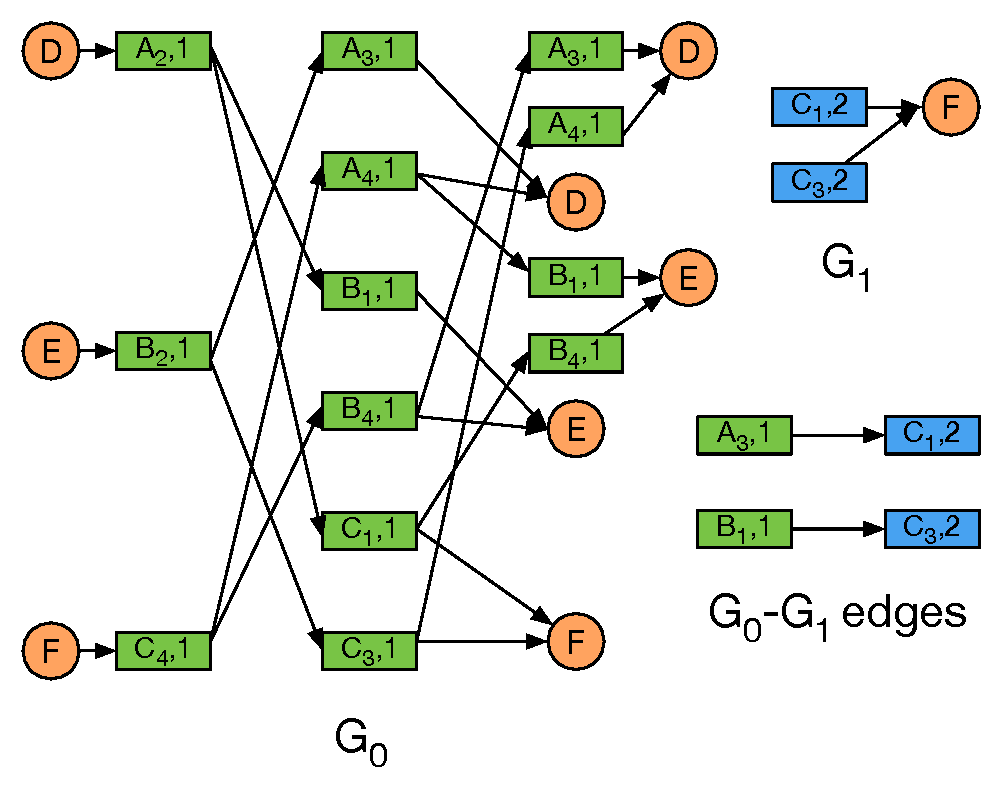
\includegraphics[width=0.48\textwidth] {figs/alo_walkthrough_c}
	\caption{Algorithm~\ref{alg:greedy} output for the example in Figure~\ref{fig:three_node}.}
	\label{fig:greedy}
\end{figure}

We use the same three-node example as the previous section, and show the output 
$G'(V', E')$ in Figure~\ref{fig:greedy}. 
We assign a new tag $t'$ (different from the brute-force tag) based on $G'(V', E')$, 
and generate switch configurations based on the algorithm output. We see that
the tags have been reduced to {\em two}.


\subsubsection{Performance Analysis}\label{subsec:caveats}

\para{Algorithm runtime}. Algorithm~\ref{alg:greedy} is efficient. Given $maxTag$ 
(denoted as $T$ below), which equals to the longest path in {\em lossless routes} and
total number of switches $S$, the brute-force tagged graph at most have $S \times T$ nodes.
Each node will be examined exactly once for checking whether $G_{tmp}$ is acyclic.
Checking whether $G_{tmp}$ is acyclic with a newly added node requires a Breath-First Search,
with runtime complexity of $O(|V_{tmp}| + |E_{tmp}|)$. $|V_{tmp}|$ is bounded by the number
os switches $S$, and $|E_{tmp}|$ is bounded by the number of links, $L$, in the network.
Therefore, the total runtime complexity is $O(S \times T \times (S+L))$.

\para{The output number of tags.} Algorithm~\ref{alg:greedy} significantly 
reduces the number of tags on topology other than Clos. For example, we 
have tested it on BCube topology without any special design for BCube. It gives the optimal 
result -- a $k$-level BCube needs $k$ tags for {\em one} lossless application 
class. In addition, we test unstructure topology like Jellyfish. The result is still promising.
\fixme{Jellyfish with 1000 nodes require only X tags. Details are in \S\ref{sec:eval}.}

\begin{figure}[t]
	%\vspace{-0.1in}
	\centering
	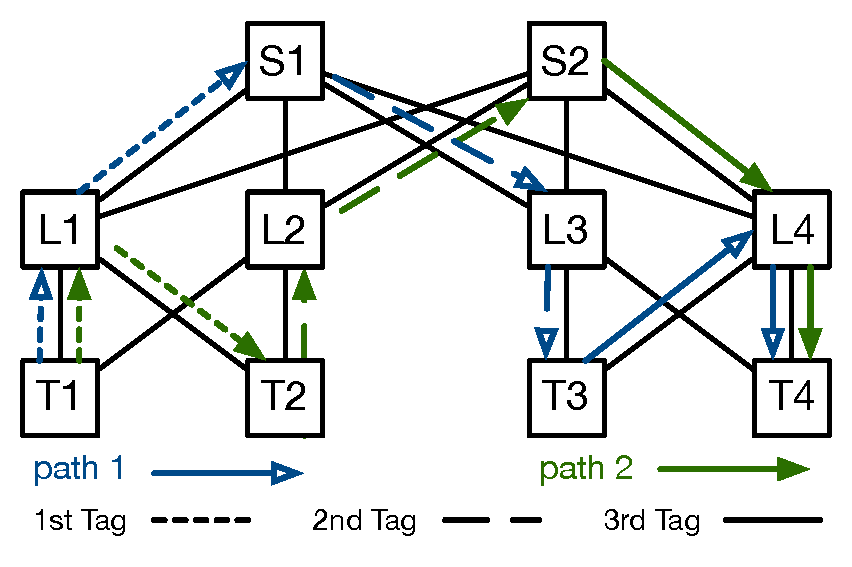
\includegraphics[width=0.48\textwidth] {figs/nonoptimal_example}
	\caption{Algorithm~\ref{alg:greedy} does not output optimal result for Clos with 1-bounce paths.}
	\label{fig:nonoptimal}
\end{figure}

However, Algorithm~\ref{alg:greedy} may not always return the optimal solution. For example, 
we again consider the simple three-layer Clos network in Figure~\ref{fig:nonoptimal}. 
Assuming ``normal'' and ``1-bounce'' packets must be lossless,  
we know the optimal tagging system only requires {\em two} lossless queues. However, the 
greedy algorithm will output {\em three} lossless queues. The reason is that 
Algorithm~\ref{alg:greedy} does not combine bounces that happen when the packet is going up
and when the packet is coming down. As a result, it has to 
assign a separate prirotiy for each case, as shown in Figure~\ref{fig:nonoptimal}.
The fundamental reason is that generic algorithm does not fully utilize the inherently 
characteristics of structured topology like Clos. 

%Second, the generic algorithm is inefficient in reusing priorities for multiple application classes.
%For example, the generic algorithm output is two priorities per application class, and the operators
%have up to two prioritie on switches. In this case, only {\em one} lossless application
%class is supported. However, if we can find a smarter tagging system that ensures basic connectivity 
%with only the first micropath, we can compress {\em two} application classes into two switch priorities, 
%as described in Section~\ref{sec:clos}.

\para{Higher bound.} Though Algorithm~\ref{alg:greedy} does not guarantee optimal result, 
it has a higher bound of the tags. Without any assumptions, the worst case 
is the same as using the brute-force solution, which require as many tags as the length of 
longest lossless route, $T$. However, if we know that the smallest cycle in lossless routes
is longer than $l$, the output number of tags is bounded by $\lceil T/l \rceil$. The proof
can be directly obtained from the greedy algorithm process, and is omitted for brevity.

\subsection{Tag Reusing}

The tag reusing for generic topology remains mostly the same as the Clos version.
The first lossless class starts with tag 0. The second lossless class starts with 
tag 1. For all tag changing rules that are for first class, {\em e.g.,} 
$(A_i, x)\rightarrow(B_j, y)$, we install another rule handling the second class,
{\em i.e.,} $(A_i, x+1)\rightarrow(B_j, y+1)$. This goes on to more lossless classes.

For Clos version, we prove that there is no deadlock even after the traffic mix among
different classes. However, with the output of Algorithm~\ref{alg:greedy}, the traffic
of differenct classes does {\em not} even mix on the same link with the same tag!
This is because, whenever the packets of class $m$ switch to tag $n$,  the packets of
class $m+1$ will switch to $n+1$. Therefore, $G_n$ of class $m$ and $G_n$ of class $m+1$
remain disconnected and cannot create a cycle.

